\documentclass[12pt]{article}
\usepackage{ifthen,empheq}
\usepackage[]{graphicx}
\usepackage[]{minted}
\usepackage{fancyhdr}
\usepackage[multidot]{grffile}
%\usepackage[]{dot2texi}
\setlength{\headheight}{20pt}
\lhead{Assignment 1}
\chead{Dilawar Singh}
\rhead{\today}

\lfoot{}\cfoot{\thepage}\rfoot{}
\pagestyle{fancy}

% Set up counters for problems and subsections

\newcounter{ProblemNum}
\newcounter{SubProblemNum}[ProblemNum]

\renewcommand{\theProblemNum}{\arabic{ProblemNum}}
\renewcommand{\theSubProblemNum}{\alph{SubProblemNum}}

\newcommand*{\anyproblem}[1]{\newpage\subsection*{#1}}
\newcommand*{\problem}[1]{\stepcounter{ProblemNum} %
   \anyproblem{Problem \theProblemNum. \; #1}}
\newcommand*{\soln}[1]{\subsubsection*{#1}}
\newcommand*{\solution}{\soln{Solution}}
\renewcommand*{\part}{\stepcounter{SubProblemNum} %
  \soln{Part (\theSubProblemNum)}}

\renewcommand{\theenumi}{(\alph{enumi})}
\renewcommand{\labelenumi}{\theenumi}
\renewcommand{\theenumii}{\roman{enumii}}

\usepackage{hyperref}

\begin{document}

\problem{}

\part
If $0<a<b$, and c is any real number, rewrite the sets $\{x: a<|x-c|<b\}$ in
terms of intervals.   Do the same for $a=0$, and also give a clear description
in words.  In this case, it will be something like "all the numbers between
[something] and [something else] except for [these one(s)]

\solution

Its usually a good idea to play with concrete numbers before manipulating the
symbols. For example, which one is correct  $a < b < c$ then $-a > -b > -c$, or
$a < b < c$ then $-a < -b < -c$  etc. This become easy to answer once we notice
that $1 < 2 < 3$ then $ -1 > -2 > -3$. This is just a quick and dirty reality
check rather than replacement of understanding by doing proof. We are going to
use this simple fact.

We have, $ \{ x : a < | x - c | < b \}$ which means $a < x - c < b,
\text{when}\; x > c$, and $a < c - x < b, \text{when}\; x < c$. The later can
be rewritten as $-a > x -c > -b$. 

For two different cases ($x > c$, and $x < c$), we have the following:
\begin{align}
    a &< x - c < b  &(a + c < x < b + c) \\
    -a &> x -c < -b &(-a +c < x < -b +c)
\end{align}

Now we can use {\bf intervals } to rewrite it i.e. $x = { (a+c, b+c) \cup
(-a+c,-b+c) }$.

\paragraph{Simulation result} See the figure \ref{fig:1a}. Code is available
\href{https://github.com/dilawar/Courses/blob/master/Calculus2016/Homework1/sol1_a.py}{here}.

\begin{figure}[ht!]
    \centering
    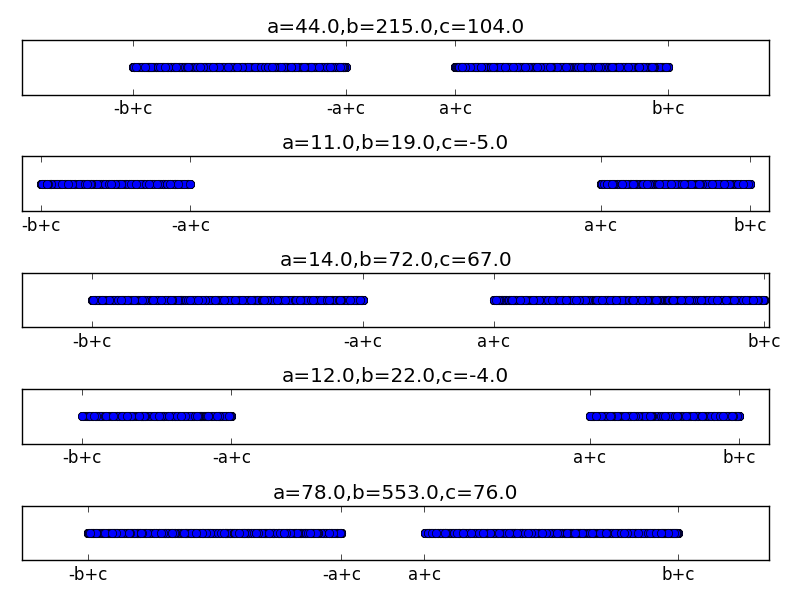
\includegraphics[width=\textwidth]{./sol1_a.py.png}
    \caption{Numerical solution to problem 1(a)}
    \label{fig:1a}
\end{figure}


\part 
Given $a<b$ real numbers, describe the intervals $(a,b)$ using the
absolute value function.  That is, write $(a,b)=\{x:  ... \}$ where "$\ldots$"
is some condition using absolute value.

\solution

$(a, b) = \{ x : x > a\; \text{and}\; x < b \}$. How about this,
$ (a, b) = \{ x  : \left| x - \frac{a+b}{2} \right| < \frac{b-a}{2} \}$.  See
the simulation result in figure \ref{fig:1b}.

\begin{figure}[ht!]
\begin{center}
    \includegraphics[width=1\textwidth]{./sol1_b.py.png}
\end{center}
\caption{Solution to solution 1(b)}
\label{fig:1b}
\end{figure}


\part

Similarly, express $\{a,b\}$, i.e. the set containing precisely the two
(different) numbers a and b (e.g. $\{-14.7, e+\pi\}$ or $\{1776,1947\}$ ) using
absolute values. 

\solution 

How about this  $ \{a, b \} = \{ x : [a, a] \cup [b,b] \}$. 

\problem{ }

\part
Show that for any $x, y$, $||x|-|y|| \le |x+y|$.  (This is a useful
counterpart to the triangle inequality and requires a very similar analysis.)

\solution 


\part
Write the set $\{x: |x^2-2x-3|>x\}$ as a union of intervals (i.e. figure out
   explicitly for which x this statement is true)




\section{Appendix}
\scriptsize
\subsection{Solution to problem 1(a)}
\inputminted{python}{./sol1_a.py}

\subsection{Solution to problem 1(b)}
\inputminted{python}{./sol1_b.py}

\end{document}          
